\documentclass[11pt,a4paper]{article}

\usepackage[utf8]{inputenc} 
\usepackage[T1]{fontenc} 
\usepackage{lmodern}
\usepackage[margin=2cm]{geometry}
\usepackage[german]{babel}
\usepackage{amsmath} 
\usepackage{graphicx} 
\usepackage{booktabs}
\usepackage{hyperref}
\hypersetup{
    colorlinks,
    citecolor=red,
    filecolor=black,
    linkcolor=black!20!blue!90!,
    urlcolor=black} 
\usepackage{nicefrac}
\usepackage[table]{xcolor}
\usepackage{tocloft}

\setlength{\parindent}{0pt}
\setlength{\parskip}{1ex plus 0.5ex minus 0.5ex}

\definecolor{incolor}{rgb}{0.0, 0.0, 0.5}

\hbadness=99999

\newcommand{\refpy}[1]{Siehe Anhang: \textit{Rechnungen in Python} (\texttt{{\color{incolor}In [{\color{incolor}#1}]}})}
\newcommand\dif{\mathop{}\!\mathrm{d}}
\newcommand{\halftime}[4]{\begin{figure}[h]
\begin{minipage}{.#1\textwidth}#3\end{minipage}\begin{minipage}{.#2\textwidth}
\centering
#4\end{minipage}
\end{figure}}
\renewcommand{\vec}{\boldsymbol}

\begin{document}

{
\centering 
\large 
Physiklabor für Anf\"anger*innen \\
Ferienpraktikum im Sommersemester 2018 \\[4mm]
\textbf{\LARGE 
Versuch 14: Streuversuch
} \\[3mm]
(durchgef\"uhrt am 01.10.2018 bei Julia M\"uller) \\
Andréz Gockel, Patrick M\"unnich\\
\today \\[10mm]
}

\vspace{50pt}
\tableofcontents
\vspace{22pt}
\listoftables
\vspace{22pt}
\listoffigures
\pagebreak

\section{Ziel des Versuchs}

Das Ziel dieses Versuchs ist es, experimentell die Streuung von Teilchen zu visualisieren, in dem man Kugeln auf ein Target schie\ss t und die Auftreffpunkte betrachtet. Hiermit wird dann mit der Abh\"angigkeit des Streuwinkels vom Sto\ss parameter der Durchmesser des Targets bestimmt.

\section{Theorie}

Wird eine Kugel mit Radius $r$ auf eine festgehaltene Kugel mit Radius $R$, auch ,,Target'' genannt, gescho\ss en, so wird sie mit dem Streuwinkel $\theta$ gestreut. $\theta$ h\"angt hier vom Sto\ss parameter $b$ ab. Zum genaueren Verst\"andnis muss eine Skizze angebracht werden:

% 2.7 

Hierzu gelten folgende Formeln:

% change overline to curved

\begin{equation}
\overline{CE}=\overline{BD}=s\arcsin\frac{b}{s}\approx b\label{eq:1}
\end{equation}
\begin{equation}
\theta=\frac{\overline{AD}}{s}\approx\frac{\overline{AB}-b}{s}\label{eq:2}
\end{equation}
\begin{equation}
\sin\beta=\frac{b}{r+R}\label{eq:3}
\end{equation}

Au\ss erdem k\"onnen wir unser $\theta$ folgenderma\ss en ausdr\"ucken:
\begin{equation}
\theta=\frac{B}{s}\label{eq:4}
\end{equation}

\section{Aufbau}

% describe set up
% insert pic name, designation, toc caption, caption, label
%\halftime{5}{5}{In diesem Versuch sind ein Streuapparat mit Plexiglasdeckel, eine Rolle druckempfindliches Papier, eine Schahtel mit Kugeln und ein Bandma\ss\ vorhanden.}{\fbox{\includegraphics[width=0.5\textwidth]{NAME}}
%   \renewcommand\thefigure{BX}
%\caption[XXXX]{XXXX \cite{Anleitung}}
%\label{Pic:X}}

\section{Durchführung}

% describe exp.
Man beginnt damit, dass das Papier an die Innenwand des Zylinder des Streuapparats gesteckt wird. Wichtig ist hier nat\"urlich, dass die druckempfindliche Seite nach innen zeigen muss.

Es werden dann f\"ur verschiedene Sto\ss parameter $b$, welche durch Bewegen des Schu\ss ger\"ats eingestellt werden, die Kugeln alle an das Target innerhalb des Streuapparats gescho\ss en. Sind alle Kugeln gescho\ss en, so wird der Sto\ss parameter ge\"andert. Zu beachten ist, dass man sowohl von rechts als auch von links schie\ss en muss.

\section{Auswertung}

F\"ur die Auswertung muss zuerst der Papierstreifen entfernt werden. Man betrachtet die Aufsto\ss punkte und mittelt sie. Hierzu beginnt man graphisch und findet rechts und links Grenzen, sodass 68\% der Punkte innerhalb der Grenzen liegen. Danach geht man analytisch vor und berechnet mit
\begin{equation}
\frac{\sum_{i=1}^n x_i}{n}\label{mean}
\end{equation}
die Mittelwerte und mit
\begin{equation}
s_{\bar{x}}=\frac{\sum{s_x}}{\sqrt{n}}\label{meanstd}
\end{equation}
deren Unsicherheiten. Wir erhalten damit folgende Werte:

\begin{table}[h]
\centering
\caption{Gemittelte Datenpunkte} \vspace{11pt}
$\begin{array}{l}
\textrm{Unsicherheiten:}\\
\textrm{B: } \pm 0.1 \textrm{cm}\\
\textrm{Position: } \pm 0.05 \textrm{cm}\\
\end{array}$
\begin{tabular}{ccc}
\toprule
\textrm{Messreihe} & \textrm{Position}/\textrm{cm} & \textrm{B}/\textrm{cm} \\
\midrule 
1 & 109.00 & 87.8 \\
2 & 108.00 & 65.0 \\
3 & 108.50 & 77.4 \\
4 & 107.50 & 49.4\\
5 & 111.50 & 64.5 \\
6 & 111.00 & 75.7\\
7 & 112.00 & 55.1 \\
8 & 111.75 & 50.2 \\
9 & 111.25 & 70.0 \\
10 & 109.25 & 70.25 \\ 
\bottomrule
\end{tabular}
\phantom{$\begin{array}{l}
\textrm{Unsicherheiten:}\\
\textrm{B: } \pm 0.1 \textrm{cm}\\
\textrm{Position: } \pm 0.05 \textrm{cm}\\
\end{array}$}
\label{Tab:1}
\end{table}

Um unsere Werte aufzutragen und den Radius $R$ zu bestimmen berechnen wir noch mit (\ref{eq:4}) die Werte f\"ur $\theta$. Wir verwenden f\"ur $s$ unser bestimmter Radius des zylindrischen Streuapparats von $(63.8\pm0.5)$\,cm und die eben berechneten Werte f\"ur die Positionen.

Um den Fehler unserer $\theta$ zu berechnen nutzen wir:
\[
\frac{\partial\theta}{\partial b}=\frac{1}{s}
\]
\[
\frac{\partial\theta}{\partial s}=-\frac{b}{s^2}
\]
\[
\Delta\theta=\sqrt{\left(\frac{\partial\theta}{\partial b}\Delta b\right)^2+\left(\frac{\partial\theta}{\partial s}\Delta s\right)^2}
\]

Wir erhalten als Werte:

\begin{table}[h]
\centering
\caption{Werte f\"ur $\theta$} \vspace{11pt}
\begin{tabular}{ccc}
\toprule
\textrm{Messreihe} & \textrm{Position}/\textrm{cm} & $\theta$ /\textrm{rad} \\
\midrule 
1 & 109.00 & $2.75\pm0.02$ \\
2 & 108.00 & $2.03\pm0.02$ \\
3 & 108.50 & $2.43\pm0.02$ \\
4 & 107.50 & $1.55\pm0.01$\\
5 & 111.50 & $2.02\pm0.02$ \\
6 & 111.00 & $2.37\pm0.02$\\
7 & 112.00 & $1.73\pm0.01$ \\
8 & 111.75 & $1.57\pm0.01$ \\
9 & 111.25 & $2.19\pm0.02$ \\
10 & 109.25 & $2.20\pm0.02$ \\ 
\bottomrule
\end{tabular}
\label{Tab:2}
\end{table}

Wir k\"onnen jetzt also unsere Werte von $b$ gegen $\cos\left(frac{\theta}{2}\right)$ auftragen. Wir f\"uhren aber zuerst noch eine lineare Regression durch. Da unsere zehnte Messung stark von den anderen Messungen dieser Messreihe abweicht, lassen wir diese raus. Aus unseren Formeln,

\begin{equation}
a=\frac{n\sum x_iy_i-\sum x_i\sum y_i}{n\sum x_i^2-(\sum x_i)^2}
\end{equation}
\begin{equation}
\Delta a=s\sqrt{\frac{n}{n\sum x_i^2-(\sum x_i)^2}},
\end{equation}
\begin{equation}
b=\frac{\sum x_i^2\sum y_i-\sum x_i\sum x_iy_i}{n\sum x_i^2-(\sum x_i)^2}
\end{equation}
\begin{equation}
\Delta b=s\sqrt{\frac{\sum x_i^2}{n\sum x_i^2-(\sum x_i)^2}}
\end{equation}
\begin{equation}
s=\sqrt{\frac{1}{n-2}\sum^n_{i=1}[y_i-(a+bx_i)]^2}
\end{equation}
interessiert uns eigentlich nur die Steigung $a$. Wir erhalten mit unserer Rechnung
\[a_{links}=-0.35\pm??\]
\[a_{rechts}=0.32\pm??\]

Das resultierende Bild sieht dann folgenderma\ss en aus:

\begin{figure}[p]
\centering
\fbox{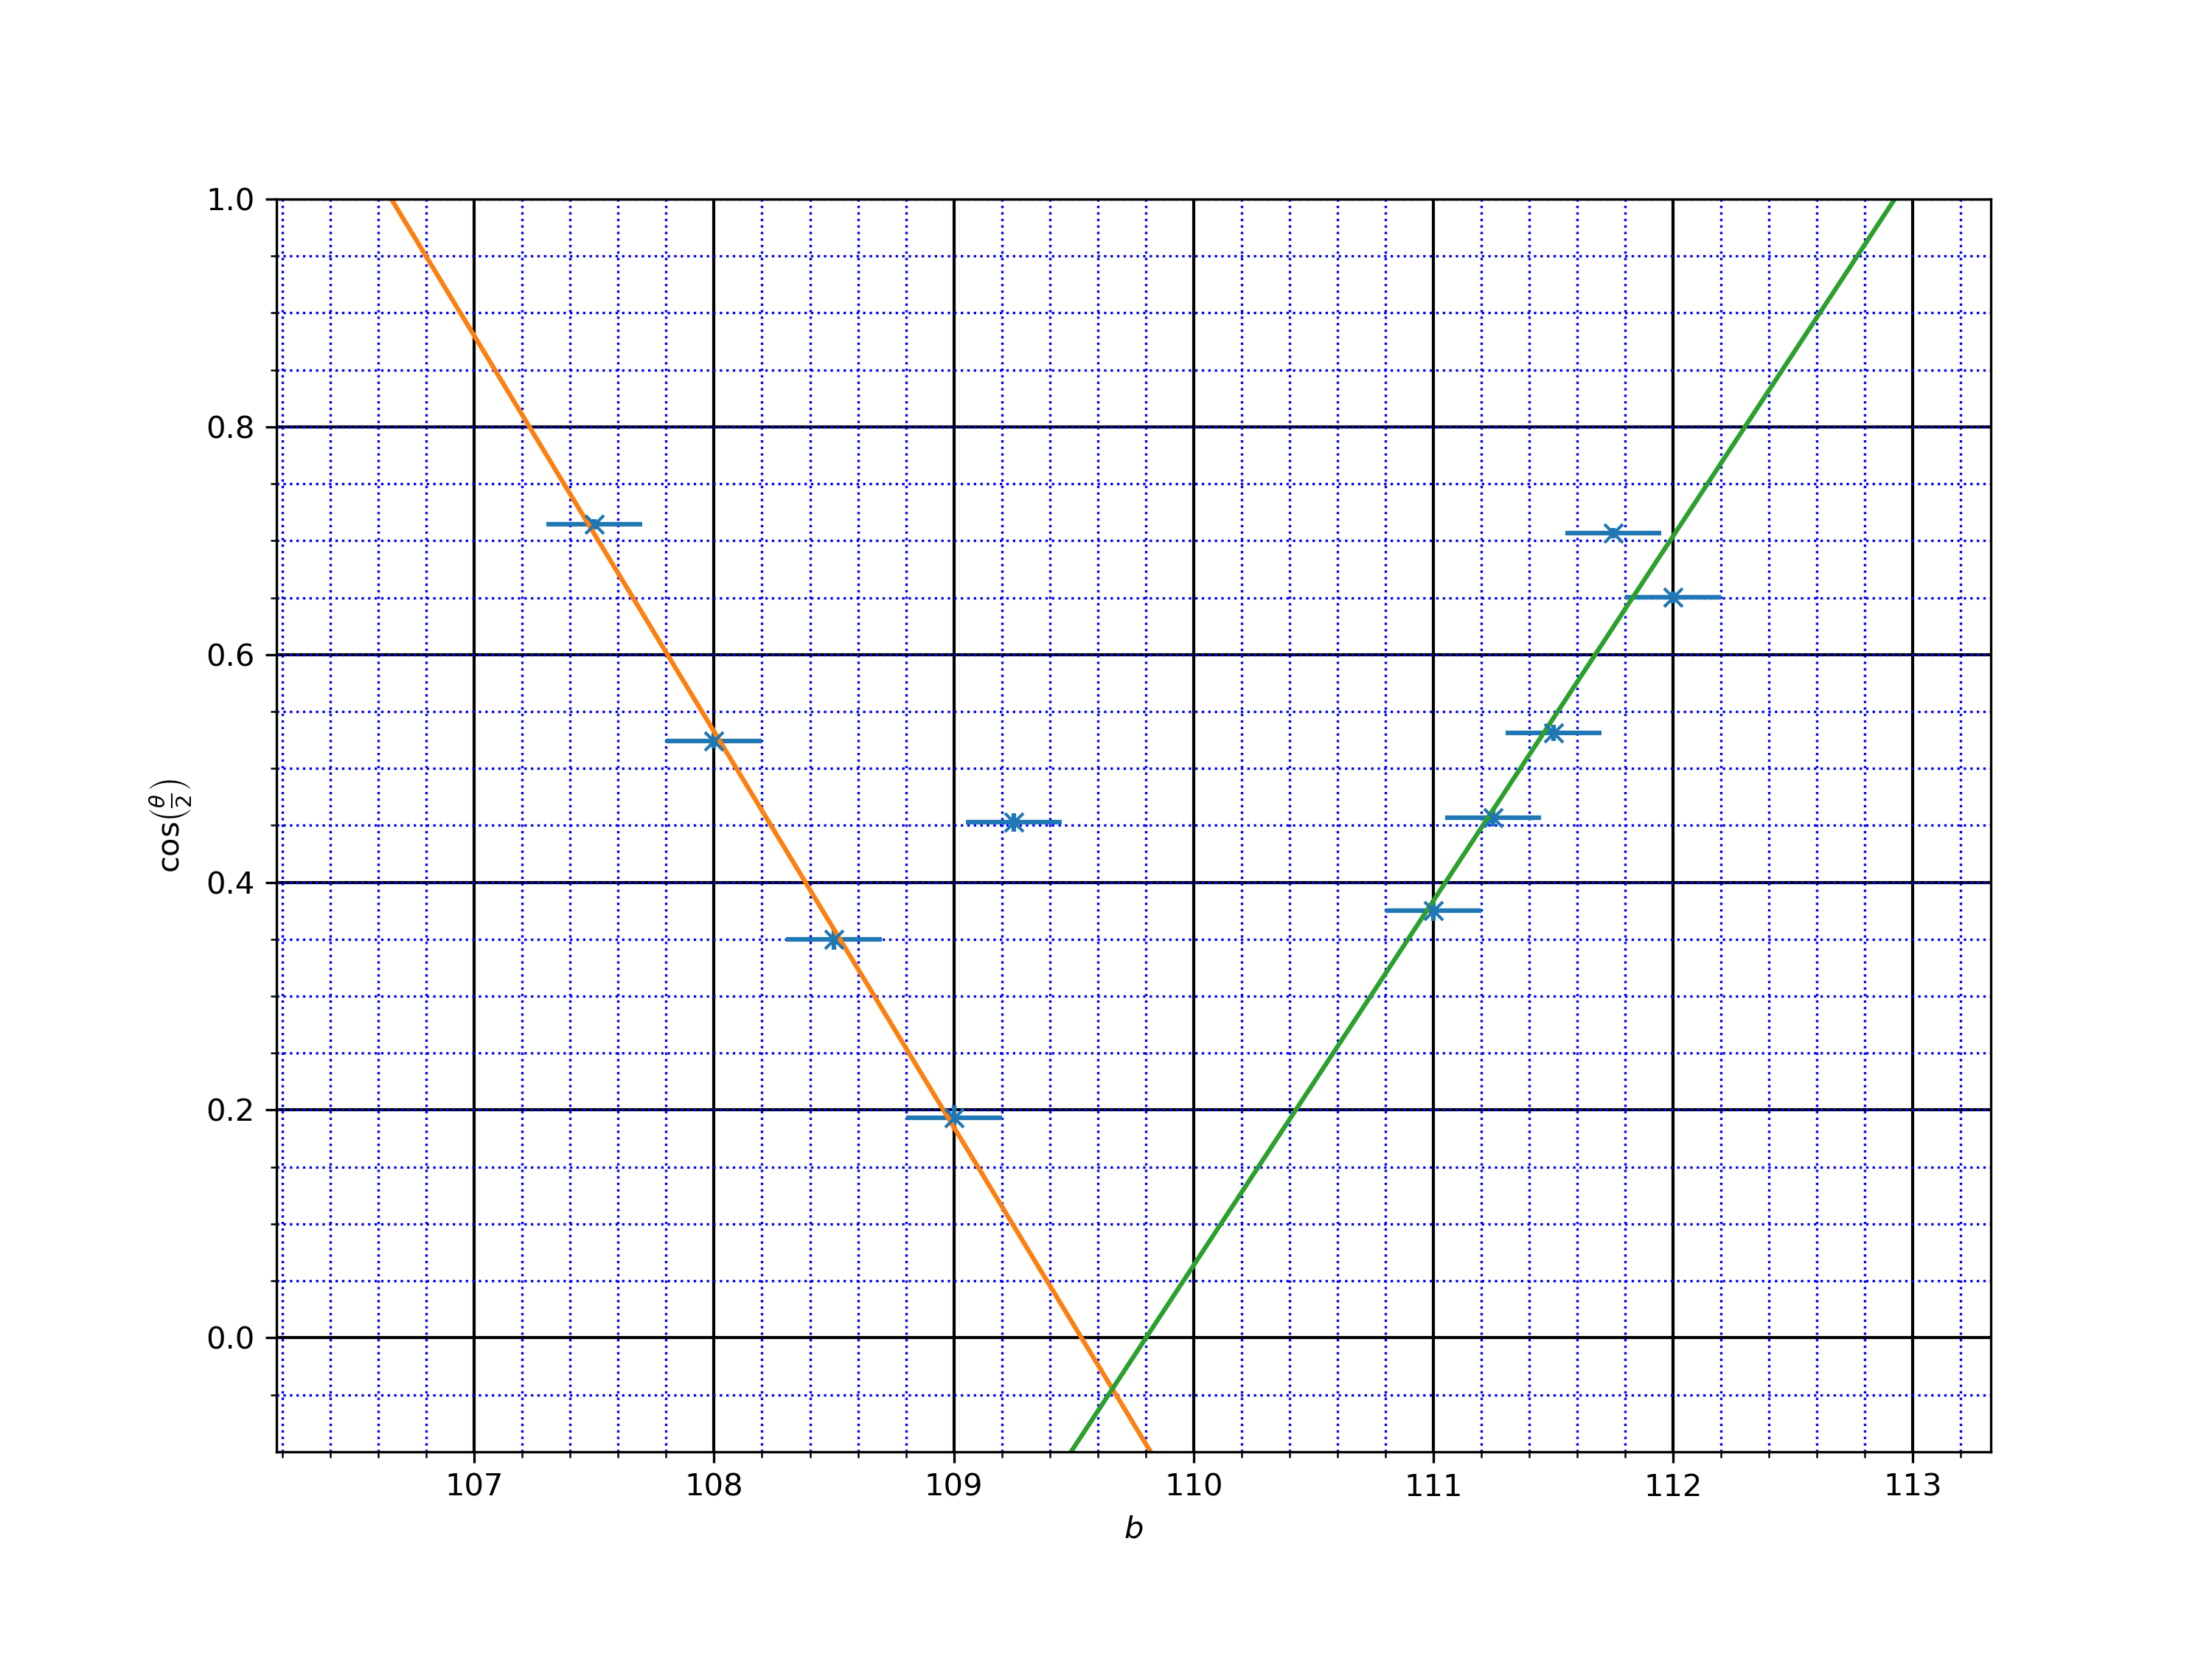
\includegraphics[width=0.8\textwidth]{graph.png}}
\renewcommand\thefigure{1}
\caption{Auftragung der Messwerte und lineare Regression}
\label{Abb:1}
\end{figure}

Fehlerbalken in $y$-Achse sind hier schwer zu erkennen, wurden jedoch berechnet. Hierzu leiten wir $\cos\left(\frac{\theta}{2}\right)$ partiell nach $\theta$ ab:
\[
\frac{\partial\cos\left(\frac{\theta}{2}\right)}{\partial\theta}=-\frac{\sin\left(\frac{\theta}{2}\right)}{2}
\]

Der Betrag dieser partielle Ableitung mit dem Fehler von $\theta$ multipliziert ist also unser Fehler in der $y$-Achse.

Da unser Verlauch klar linear ist k\"onnen wir $\frac{1}{r+R}$ aus (\ref{eq:3}) der Steigung gleichsetzen. Wir rechnen also

\begin{equation}
\frac{1}{a}-r=R\label{eq:5}
\end{equation}

Da wir einen Fehler auf $a$ haben m\"ussen wir wieder gau\ss sche Fehlerfortpflanzung anwenden und erhalten

\[
\frac{\partial R}{\partial a}=-\frac{1}{a^2}
\]
\[
\Delta R=\left|\frac{\partial R}{\partial a}\Delta a\right|
\]

Mit unseren beiden Steigungen und dem vorgegebenen Radius der Kugeln, $2r=4.35\,\mathrm{mm}$, erhalten wir als Werte f\"ur den Radius unseres Targets:
\[r_1=2.66\pm??\]
\[r_2=2.91\pm??\]

Der Mittelwert hiervon mit (\ref{mean}) und (\ref{meanstd}) ist dann:

\[\bar{r}=2.78\pm??\]

\section{Diskussion}

XXXX

\pagebreak

\section{Anhang: Tabellen und Diagramme}

\begin{table}[h]
\centering
\caption{XXXX} \vspace{11pt}
$\begin{array}{l}
\textrm{Unsicherheiten:}\\
\textrm{XXXX: } \pm XX \textrm{XX}\\
\end{array}$
\begin{tabular}{ccc}
\toprule
\textrm{XXXX}/\textrm{XX} & \textrm{XXXX}/\textrm{XX} & \textrm{XXXX}/\textrm{XX} \\
\midrule 
2 & 0.26 & 0.23\\
\hline
4 & 0.33 & 0.25\\
\hline 
5 & & 0.3\\
\hline 
6 & 1.25 & 0.83\\
\hline 
8 & 3.9 & 0.83\\ 
\hline
9 & 4.75 & 4.6\\ 
\hline
10 & 4.7 &\\ 
\bottomrule
\end{tabular}
\phantom{$\begin{array}{l}
\textrm{Unsicherheiten:}\\
\textrm{XXXX: } \pm XX \textrm{XX}\\
\end{array}$}
\label{Tab:X}
\end{table}

%\begin{figure}[p]
%\centering
%\fbox{\includegraphics[width=0.8\textwidth]{NAME}}
%\renewcommand\thefigure{BX}
%\caption[XXXX]{XXXX}
%\label{Abb:X}
%\end{figure}

\begin{thebibliography}{9}
\bibitem{Uncertainties}''Correlations between variables are automatically handled, which sets this module apart from many existing error propagation codes.'' - https://pythonhosted.org/uncertainties/
\bibitem{Anleitung} Physikalisches Institut der Albert-Ludwigs-Universität Freiburg (Hrsg.) (08/2018): Versuchsanleitungen zum Physiklabor für Anfänger*innen, Teil 1, Ferienpraktikum im Sommersemester 2018.
\end{thebibliography}

\end{document}